\section{System Overview and Preliminaries}
\label{sec:system}
\textsc{Synopsis} is a distributed sketch constructed over voluminous spatiotemporal data streams.
The number of sketchlets (executing on different machines) that comprise the distributed sketch varies dynamically as the system scales in or out to cope with data arrival rates and memory pressure.
%Each sketchlet is responsible for one or more geographical scopes and is implemented as a stateful stream processing node that can build and retain state over time.
\textsc{Synopsis} assimilates, organizes, and compacts spatiotemporal data streams that comprise the sketch.
A stream partitioning scheme, based on the Geohash algorithm, is used to route packets to the appropriate sketchlet.
Sketchlets process stream packets emitted by stream ingesters and construct compact, in-memory representations of the observational data by extracting metadata from stream packets.
During dynamic scaling, the geographic extents managed by a sketchlet vary.
%
\vspace{0.7em}\\
%
\textbf{System Components}:
\textsc{Synopsis} relies on a set of auxiliary services that are needed to construct, update, and maintain the sketch, as well as adapt to changing system conditions:
\begin{description}[leftmargin=*]
\item[Control plane] is responsible for orchestrating control messages exchanged between sketchlets as part of various distributed protocols such as dynamic scaling.
    It is decoupled from the generic data plane to ensure higher priority and low latency processing without being affected by buffering delays and backpressure experienced during stream processing.

\item[Gossip subsystem] is used by the sketchlets to gossip about their state periodically (based on time intervals and the number of pending updates) as well as when a change in state occurs to establish an approximate global view of the system. \textsc{Synopsis} supports \emph{eventual consistency} with respect to these updates given their propagation and convergence delays.

\item[Querying subsystem] is responsible for the distributed evaluation of queries.
    This involves forwarding queries to relevant sketchlets; in some cases, multiple sketchlets may be involved based on the geographical scope of the query.

\item[Monitoring subsystem] probes sketchlets comprising \textsc{Synopsis} periodically to gather metrics that impact performance of the system.
    These include memory utilization and backlog information based on packet arrival rates and updates to the in-memory structures.
    This information is used for dynamic scaling recommendations as explained in Sections~\ref{subsec:scaling-out} and \ref{subsec:scaling-in}.
\end{description}
%
\textbf{Data Model}:
While designing \textsc{Synopsis}, we targeted a data model wherein observations are geotagged and have chronological timestamps indicating where and when the observations were made. Location information is encoded as $\langle latitude, longitude \rangle$ tuples. Observations contain multiple features (temperature, humidity, wind speed, etc.), and may be encoded as $\langle feature\_name, value \rangle$ tuples or may have predefined positions within the serialized data representation. 
%
\vspace{0.7em}\\
%
\textbf{Query Support}:
\textsc{Synopsis} supports common query constructs such as selects or joins, while also providing rich analytical queries that report statistical information, make predictions, or produce synthetic datasets (detailed fully in \S\ref{subsec:query-eval}). A key innovation in our query support is that portions of the sketch itself can be retrieved and manipulated by clients. The following query demonstrates this functionality, where climate features are requested from a region when the wind speed is more than a standard deviation away from the mean:

\begin{lstlisting}[language=SQL,style=custompy]
   SELECT location, precipitation, humidity
   WHERE location LIKE 'dj%' AND
       (wind_sp > MEAN(wind_sp) + STD(wind_sp)
       OR wind_sp < MEAN(wind_sp) - STD(wind_sp))
\end{lstlisting}
%
%\vspace{0.7em}\\
%
\textbf{Stream Partitioning}:
We use the Geohash~algorithm~\cite{geohash} to balance load and partition incoming data streams. Geohash divides the earth into a hierarchy of bounding boxes identified by Base 32 strings; the longer the geohash string, the more precise the bounding box. Figure~\ref{fig:geohash} illustrates this hierarchy. Most of the eastern United States is contained within the bounding box described by geohash \emph{D}, while \emph{DJ} encompasses substantial parts of Florida, Georgia, and Alabama. The bounding box \emph{DJKJ} (highlighted in red) contains Tallahassee, Florida. This hierarchical representation enables \textsc{Synopsis} to cope with both low- and high-density regions: several sketchlets may be tasked with managing streams originating in and around large cities, while rural areas fall under the purview of a single node.

Each bit added to a geohash string reduces its scope by half, with each character represented by five bits ($2^5 = 32$). In other words, a four-character geohash string represents 20 spatial subdivisions applied recursively to each resulting region. This property allows us to manage and allocate resources across a variety of observational densities.

\begin{figure}[h!]
    \centerline{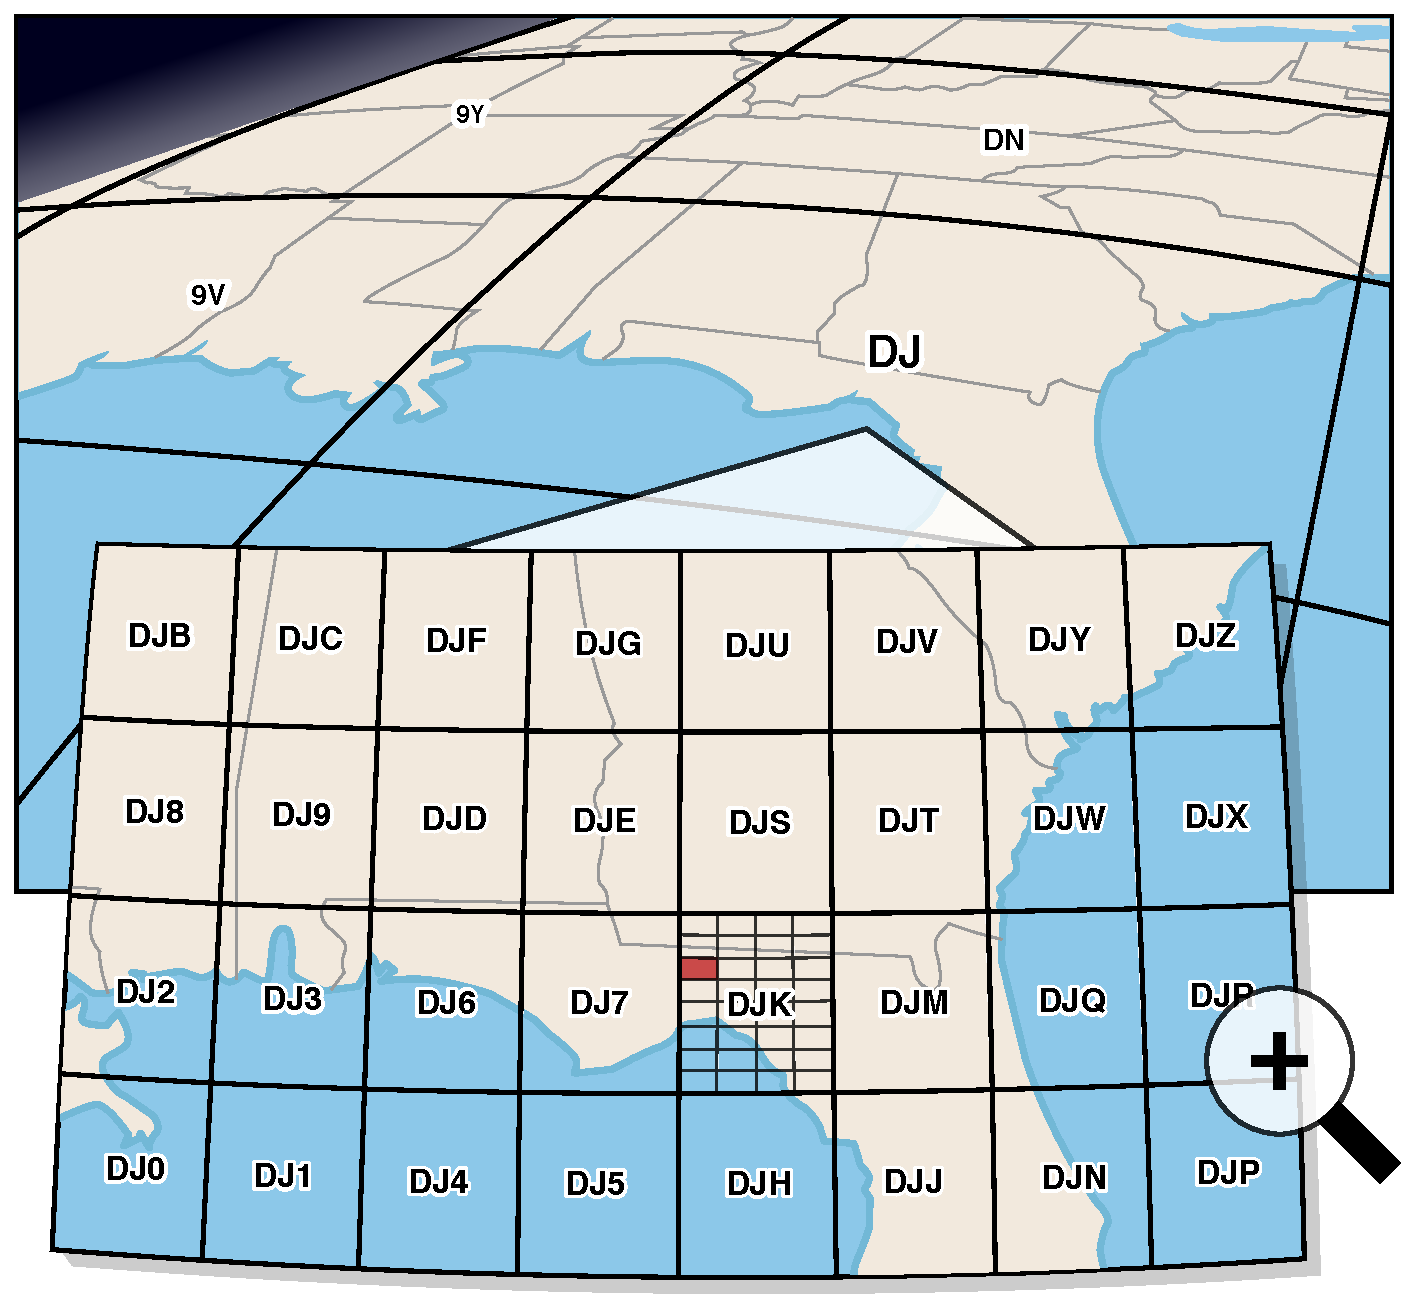
\includegraphics[width=2.5in]{figures/geohash.pdf}}
    \caption{Visual demonstration of the Geohash algorithm.}
    \label{fig:geohash}
\end{figure}


